\begin{name}
	{\tenchude}{ĐỀ ÔN TẬP SỐ 10}{LỚP TOÁN THẦY PHÁT}{\thoigian}
\end{name}
\setcounter{ex}{0}
\setcounter{bt}{0}
\Opensolutionfile{ans}[ans/ans-Vted-20-2023]
%%==========Câu 1
\begin{ex}%[2H2Y1-2]
Công thức tính diện tích xung quanh của hình trụ tròn xoay có bán kính đáy $r$ và độ dài đường sinh $l$ là
\choice
{$S_{\text{xq}}=rl$}
{\True $S_{\text{xq}}=2 \pi rl$}
{$S_{\text{xq}}=\pi rl$}
{$S_{\text{xq}}=2 \pi l$}
\loigiai{
Diện tích xung quanh của hình trụ tròn xoay có bán kính đáy $r$ và độ dài đường sinh $l$ là $S_{\text{xq}}=2 \pi rl$.
}
\end{ex}
%%==========Câu 2
\begin{ex}%[1D3Y4-1]
Cấp số nhân $\left(u_n\right)$ có $u_1=-1$, công bội $q=3$ thì $u_3$ bằng
\choice
{$5$}
{$27$ }
{$8$}
{\True $-9$}
\loigiai{
Cấp số nhân $\left(u_n\right)$ có $u_1=-1$, công bội $q=3$ thì $u_3 = u_1 \cdot q^2 = (-1)\cdot3^2 = -9$. 
}
\end{ex}
%%==========Câu 3
\begin{ex}%[2D3Y2-1]
Biết $\displaystyle\int_0 ^{1} f(x) \mathrm{\,d}x=-3$ và $\displaystyle\int_0 ^{1} g(x) \mathrm{\,d}x=4$, khi đó $\displaystyle\int_0 ^{1} (f(x)-g(x)) \mathrm{\,d}x$ bằng
\choice
{\True $-7$}
{$7$}
{$-12$}
{$1$}
\loigiai{
Ta có $\displaystyle\int_0 ^{1} (f(x)-g(x)) \mathrm{\,d}x =\displaystyle\int_0 ^{1} f(x) \mathrm{\,d}x - \displaystyle\int_0 ^{1} g(x) \mathrm{\,d}x = -3-4 = -7$.
}
\end{ex}
%%==========Câu 4
\begin{ex}%[2D1Y2-2]
\immini{Cho hàm số $f(x)$ có đồ thị như hình vẽ bên.
Hàm số đã cho đạt cực đại tại điểm
\choice
{$x=1$}
{\True $x=0$}
{$x=5$}
{$x=2$}}{\begin{tikzpicture}[scale=0.7, font=\footnotesize, line join=round, line 
	cap=round, >=stealth,
	declare function={
	f(\x)=-(\x)^3 +3*(\x)^2+1 ;
	}
	]
	%	\draw[gray!10] (-1,-1) grid (5,5);
	\draw[->] (-1,0)--(5,0) node[below]{$x$};
	\draw[->] (0,-1)--(0,6) node[left]{$y$};
	\fill (2,0) node[below]{$2$} circle(1.5pt);
	\fill (0,0) node[below left]{$O$} circle(1.5pt);
	\fill (0,1) node[below right]{$1$} circle(1.5pt);
	\fill (0,5) node[below right]{$5$} circle(1.5pt);
	\draw[dashed] (2,0)--(2,5)--(0,5);
	\draw[smooth,red] plot[domain=-1.1:3.2] ({\x},{f(\x)});
\end{tikzpicture}}
\loigiai{
Dựạ vào đồ thị, hàm số đạt cực tiểu tại điểm $x=0$.
}
\end{ex}
%%==========Câu 5
\begin{ex}%[2D4Y1-1]
Trên mặt phẳng tọa độ $Oxy$, điểm biểu diễn số phức $z=2-3 i$ có tọa độ là
\choice
{$(3 ; 2)$}
{$(3 ;-2)$}
{$(-2 ; 3)$}
{\True $(2 ;-3)$}
\loigiai{
Điểm biểu diễn số phức $z=2-3i$ có tọa độ là $(2 ;-3)$.
}
\end{ex}
%%==========Câu 6
\begin{ex}%[2D1Y4-1]
Tiệm cận ngang của đồ thị hàm số $y=\dfrac{2 x+1}{1-x}$ là
\choice
{ $y=1$}
{$y=2$}
{$y=-1$}
{\True $y=-2$}
\loigiai{
Tiệm cận ngang của đồ thị hàm số $y=\dfrac{2 x+1}{1-x}$ là $y=-2$.
}
\end{ex}
%%==========Câu 7
\begin{ex}%[2D4Y2-1]
Cho số phức $z=3-2i$. Khi đó $(1+2i)z$ có phần ảo bằng
\choice
{$7$}
{$4$}
{\True $4i$}
{$7i$}
\loigiai{
Ta có số phức $z=3-2i$, khi đó $(1+2i)z=(1+2i)(3-2 i)=3-2i+6i-4i^2=7+4i$ có phần ảo bằng $4i$.
}
\end{ex}
%%==========Câu 8
\begin{ex}%[2D2Y3-1]
Với $a$ là số thực dương tùy ý, $\log _3\left(a^4\right)$ bằng
\choice
{$4+\log _3 a$}
{$\dfrac{1}{4}+\log _3 a$}
{\True $4 \log _3 a$}
{$\dfrac{1}{4} \log _3 a$}
\loigiai{
Với $a$ là số thực dương tùy ý, $\log _3\left(a^4\right)=4 \log _3 a$.
}
\end{ex}
%%==========Câu 9
\begin{ex}%[2H3Y2-2]
Trong không gian $Oxyz$, mặt phẳng nào dưới đây có một véc-tơ pháp tuyến là $\vec{n}=(1 ; 2 ;-3)$ ?
\choice
{\True $x+2y-3z-1=0$}
{$x+2y+3z+1=0$}
{$x-2y+3z-3=0$}
{$2x-3y+z+1=0$}
\loigiai{
Mặt phẳng $x+2y-3z-1=0$ có một véc-tơ pháp tuyến là $\vec{n}=(1 ; 2 ;-3)$.
}
\end{ex}
%%==========Câu 10
\begin{ex}%[2D2Y5-1]
Nghiệm của phương trình $\log _4(2 x)=3$ là
\choice
{$x=6$}
{$x=\dfrac{7}{2}$}
{\True $x=32$}
{$x=64$}
\loigiai{
Nghiệm của phương trình $\log _4(2 x)=3 \Leftrightarrow 2x=4^3 \Leftrightarrow x=32$. 
}
\end{ex}
\begin{ex}%[]%[2H1Y2-1]
	Thể tích của một khối chóp có diện tích đáy bằng $3a^2$, chiều cao bằng $4a$ là
	\choice
	{ $12 a^3$}
	{\True $4 a^3$}
	{$3 a^3$}
	{$6 a^3$}
	\loigiai{
	$$V_{\text{Chóp}}=\dfrac{1}{3}\cdot h\cdot S=\dfrac{1}{3}\cdot 4a\cdot 3a^2=4a^3.$$
	}
\end{ex}
%%==========Câu 12
\begin{ex}%[]%[2H3Y3-3]
	Trong không gian $O x y z$, điểm nào dưới đây thuộc đường thẳng $d: \dfrac{x+1}{2}=\dfrac{y-1}{3}=\dfrac{z-2}{-1} ?$
	\choice
	{$M(2 ; 3 ;-1)$}
	{$N(1 ;-1 ;-2)$}
	{$P(-1 ;-1 ;-2)$}
	{\True $Q(-1 ; 1 ; 2)$}
	\loigiai{
	Với $x=-1;y=1;z=2$ thì $$\dfrac{x+1}{2}=\dfrac{y-1}{3}=\dfrac{z-2}{-1}=0.$$
	}
\end{ex}
%%==========Câu 13
\begin{ex}%[]%[2D1Y1-2]
	Cho hàm số $y=f(x)$ có bảng biến thiên như hình vẽ:
	\begin{center}
	
\begin{tikzpicture}
	\tkzTabInit[nocadre=false,lgt=1.2,espcl=2.5,deltacl=0.6]
	{$x$ /0.6,$y’$ /0.6,$y$ /2}
	{$-\infty$,$1$,$3$,$+\infty$}
	\tkzTabLine{,+,0,-,0,+,}
	\tkzTabVar{-/$-\infty$,+/$2$,-/$-2$,+/$+\infty$}
	\end{tikzpicture}
	\end{center}
	Hàm số đã cho nghịch biến trên khoảng nào dưới đây?
	\choice
	{$(-\infty ; 2)$}
	{$(1 ;+\infty)$}
	{$(-\infty ; 1)$}
	{\True$(1 ; 3)$}
	\loigiai{
	Ta có: $y'<0 \,\forall x \in (1;3)$ nên hàm số nghịch biến trên $(1;3)$. 
	}
\end{ex}
%%==========Câu 14
\begin{ex}%[]%[2D3Y1-1]
	Họ nguyên hàm của hàm số $f(x)=\sin 3 x$ là
	\choice
	{\True $-\dfrac{1}{3} \cos 3 x+C$}
	{$-\cos 3 x+C$}
	{$\cos 3 x+C$}
	{$\dfrac{1}{3} \cos 3 x+C$}
	\loigiai{
	Ta có $$\displaystyle\int \sin 3x \mathrm{\,d}x= \dfrac{1}{3} \displaystyle\int \sin 3x \mathrm{\,d}(3x) = \dfrac{-1}{3} \cos 3x $$ 
	}
\end{ex}
%%==========Câu 15
\begin{ex}%[]%[2D1Y3-1]
	Cho hàm số $f(x)$ có đồ thị như hình vẽ bên:
	\begin{center}
	\begin{tikzpicture}[scale=0.8, font=\footnotesize, line join=round, line cap=round,>=stealth]
	%\def\a{1} \def\b{-4} \def\c{3} % Hệ số
	\def\xmin{-4} \def\xmax{3.5}
	\def\ymin{-2.2} \def\ymax{5} 
	%\draw[color=gray!50,dashed] (\xmin,\ymin) grid (\xmax,\ymax); 
	\draw[->] (\xmin,0)--(\xmax,0) node [below]{$x$};
	\draw[->] (0,\ymin)--(0,\ymax) node [left]{$y$};
	\node at (0,0) [below left]{$O$};
	\clip (\xmin+0.1,\ymin+0.1) rectangle (\xmax-0.1,\ymax-0.1);
	\draw[smooth,samples=300] plot(\x,{0.1449431341897098*(\x)^(5.0)-0.32673519077246793*(\x)^(4.0)-0.7400913139938888*(\x)^(3.0)+1.2180720180035751*(\x)^(2.0)+0.11947416457398054*(\x)+1.32});
	\draw[dashed,thin] (-1.55,3.6)--(-1.55,0) (0,1.3)--(1.4,1.3)--(1.4,0);
	\draw (-1.55,-0.2) node {$-3$};
	\draw (1.4,0.4) node[anchor=north west] {$2$};
	\draw (-0.3,1.72) node[anchor=north west] {$2$};
	\draw (2.86,0.4) node[anchor=north west] {$4$};
	\end{tikzpicture}
	\end{center}
	Giá trị lớn nhất của hàm số đã cho trên đoạn $[-3 ; 4]$ bằng
	\choice
	{$f(2)$}
	{\True $f(-3)$}
	{$f(4)$}
	{$f(0)$}
	\loigiai{
	Dựa vào đồ thị ta có: $\max\limits_{[-3;4]} f(x)=f(-3)$.
	}
\end{ex}
%%==========Câu 16
\begin{ex}%[2H1Y3-2]
	Cho khối hộp đứng có đáy là hình vuông cạnh bằng $a$, độ dài cạnh bên bằng $3a$. Thể tích của khối hộp đã cho bằng
	\choice
	{$9a^3$}
	{$a^3$}
	{\True $3a^3$}
	{$\dfrac{1}{3}a^3$}
	\loigiai{
	Theo đề bài ta có:\\
	Đáy là hình vuông cạnh bằng $a$ nên diện tích đáy $B=a^2$.\\
	Độ dài cạnh bên bằng $3a$ nên chiều cao $h=3a$.\\
	Suy ra $V=Bh=a^2\cdot 3a=3a^3$.
	}
\end{ex}
%%==========Câu 17
\begin{ex}%[2D2Y5-1]
	Tập nghiệm của bất phương trình $2^{1-x}\ge 2$ là
	\choice
	{$\left(0;+\infty\right)$}
	{$\left[0;+\infty\right)$}
	{$\left(-\infty;0\right)$}
	{\True $\left(-\infty;0\right]$}
	\loigiai{
	Ta có $2^{1-x}\ge 2\Leftrightarrow 1-x\ge 1\Leftrightarrow x\le 0$.\\
	Vậy tập nghiệm của bất phương trình là $\left(-\infty;0\right]$.
	}
\end{ex}
%%==========Câu 18
\begin{ex}%[1D2Y2-1]
	Có bao nhiêu số tự nhiên gồm năm chữ số đôi một phân biệt được thành lập từ các chữ số $1, 2, 3, 4, 5$?
	\choice
	{$5^5$}
	{$\mathrm{A}_5^1$}
	{\True$5!$}
	{$\mathrm{C}_5^1$}
	\loigiai{
	Số các số tự nhiên gồm năm chữ số đôi một phân biệt được thành lập từ các chữ số $1, 2, 3, 4, 5$ là số hoán vị của $5$ phần tử. Vậy có $5!$ số.
	}
\end{ex}
%%==========Câu 19
\begin{ex}%[2D3Y2-1]
	Biết $\displaystyle\int\limits_0^1 f(x) \mathrm{\,d}x=-2$ và $\displaystyle\int\limits_1^5 f(x) \mathrm{\,d}x=3$, khi đó $\displaystyle\int\limits_0^5 2f(x) \mathrm{\,d}x$ bằng
	\choice
	{\True$2$}
	{$10$}
	{$6$}
	{$-4$}
	\loigiai{
	Ta có $\displaystyle\int\limits_0^5 2f(x) \mathrm{\,d}x=2\displaystyle\int\limits_0^5 f(x) \mathrm{\,d}x=2\left[\displaystyle\int\limits_0^1 f(x) \mathrm{\,d}x+\displaystyle\int\limits_1^5 f(x) \mathrm{\,d}x \right]=2\left(-2+3\right)=2$.
	}
\end{ex}
%%==========Câu 20
\begin{ex}%[2D4Y3-1]
	Cho hai số phức $z_1=1+2i$ và $z_2=1-i$. Số phức $\dfrac{z_1}{z_2}$ bằng
	\choice
	{\True$-\dfrac{1}{2}+\dfrac{3}{2}i$}
	{$\dfrac{1}{2}-\dfrac{3}{2}i$}
	{$-1+3i$}
	{$\dfrac{3}{2}-\dfrac{1}{2}i$}
	\loigiai{
	Ta có $\dfrac{z_1}{z_2}=\dfrac{1+2i}{1-i}=\dfrac{\left(1+2i\right)\left(1+i\right)}{\left(1-i\right)\left(1+i\right)}=\dfrac{-1+3i}{2}=-\dfrac{1}{2}+\dfrac{3}{2}i$.
	}
\end{ex}
%%==========Câu 21
\begin{ex}%[2H3Y1-1]
	Trong không gian $Oxyz$, cho véc-tơ $\overrightarrow{a}=(-3;2;1)$ và điểm $A(4;6;-3)$, tọa độ điểm $B$ thỏa mãn $\overrightarrow{AB}=\overrightarrow{a}$ là
	\choice
	{$\left(7;4;-4\right)$}
	{$\left(-1;-8;2\right)$}
	{\True $\left(1;8;-2\right)$}
	{$\left(-7;-4;4\right)$}
	\loigiai{
	Ta có $\overrightarrow{OB}=\overrightarrow{AB}+\overrightarrow{OA}=\left(1;8;-2\right)$.
	}
\end{ex}
%%==========Câu 22
\begin{ex}%[2D3Y2-1]
	Nếu $f(3)=2$ và $\displaystyle\int\limits_1^3 f'(x) \mathrm{\,d}x=6$ thì $f(1)$ bằng
	\choice
	{$4$}
	{\True $-4$}
	{$8$}
	{$3$}
	\loigiai{
	$\displaystyle\int\limits_1^3 f'(x) \mathrm{\,d}x=6 \Leftrightarrow f(x)\bigg|_1^3=6 \Leftrightarrow f(3)-f(1)=6 \Leftrightarrow f(1)=f(3)-6=2-6=-4$.
	}
\end{ex}
%%==========Câu 23
\begin{ex}%[2D1Y5-1]
	\immini{
	Đồ thị của hàm số nào dưới đây có dạng như hình vẽ bên?
	\choice
	{$y=x^4-4x^2$}
	{\True $y=-x^4+4x^2$}
	{$y=-x^3+2x$}
	{$y=x^3-2x$}	
	}
	{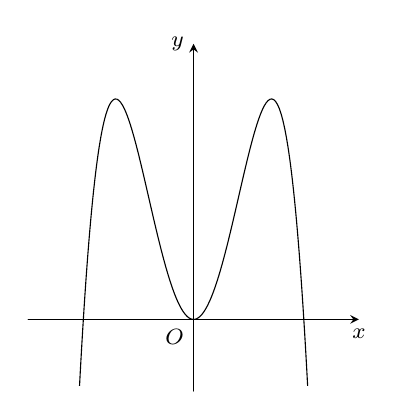
\begin{tikzpicture}[scale=.7,>=stealth, font=\footnotesize, line join=round, line cap=round]
	\def\a{-1} \def\b{4} \def\c{0} % Hệ số
	\def\xmin{-3} \def\xmax{3}
	\def\ymin{-1.3} \def\ymax{5} 
	%\draw[color=gray!50,dashed] (\xmin,\ymin) grid (\xmax,\ymax); 
	\draw[->] (\xmin,0)--(\xmax,0) node [below]{$x$};
	\draw[->] (0,\ymin)--(0,\ymax) node [left]{$y$};
	\node at (0,0) [below left]{$O$};
	\clip (\xmin+0.1,\ymin+0.1) rectangle (\xmax-0.5,\ymax-0.1);
	\draw[smooth,samples=300] plot(\x,{\a*(\x)^4+\b*(\x)^2+\c});
	\end{tikzpicture}}
	\loigiai{
	Dựa vào đồ thị của hàm số ta loại $y=x^4-4x^2$, $y=-x^3+2x$, $y=x^3-2x$ và chọn $y=-x^4+4x^2$.
	}
\end{ex}
%%==========Câu 24
\begin{ex}%[2D1Y5-4]
	Đồ thị hàm số $y=\dfrac{1-x}{x+1}$ cắt trục tung tại điểm có tọa độ là
	\choice
	{$\left(0;-1\right)$}
	{\True $\left(0;1\right)$}
	{$\left(1;0\right)$}
	{$\left(1;1\right)$}
	\loigiai{
	Cho $x=0 \Rightarrow y=1$. Suy ra đồ thị hàm số $y=\dfrac{1-x}{x+1}$ cắt trục tung tại điểm có tọa độ là $\left(0;1\right)$.
	}
\end{ex}
%%==========Câu 25
\begin{ex}%[2H3Y1-3]
	Trong không gian $Oxyz$, phương trình mặt cầu có tâm $I(2;1;2)$ bán kính bằng $3$ là
	\choice
	{$\left(x+2\right)^2+\left(y+1\right)^2+\left(z+2\right)^2=3$}
	{$\left(x-2\right)^2+\left(y-1\right)^2+\left(z-2\right)^2=3$}
	{$\left(x+2\right)^2+\left(y+1\right)^2+\left(z+2\right)^2=9$}
	{\True $\left(x-2\right)^2+\left(y-1\right)^2+\left(z-2\right)^2=9$}
	\loigiai{
	Phương trình mặt cầu có tâm $I(2;1;2)$ bán kính bằng $3$ là $\left(x-2\right)^2+\left(y-1\right)^2+\left(z-2\right)^2=9$.
	}
\end{ex}
%%==========Câu 26
\begin{ex}%[2D2B4-1] 
	Tập xác định của hàm số $y=\log (3-x)$ là
	\choice
	{$(0;3)$}
	{$(3;+\infty)$}
	{\True $(-\infty; 3)$}
	{$(-3;+\infty)$}
	\loigiai{
	Hàm số $y=\log (3-x)$ xác định khi $3-x>0 \Leftrightarrow x<3$.
	}
\end{ex}
%%==========Câu 27
\begin{ex}%[2H2B1-1] 
	Một khối cầu có thể tích bằng $\dfrac{9 \pi}{2}$ thì đường kính của nó bằng 
	\choice
	{\True $\dfrac{3}{2}$}
	{$\dfrac{2}{3}$}
	{$\dfrac{4}{3}$}
	{$3$}
	\loigiai{
	$V=\dfrac{4}{3} \pi R^3 \Rightarrow \dfrac{9 \pi}{2 }=\dfrac{4}{3} \pi R^3 \Rightarrow R^3=\dfrac{27}{8}\Rightarrow R=\dfrac{3}{2}$.
	}
\end{ex}
%%==========Câu 28
\begin{ex}% [2D2B4-3] 
\immini{Trên khoảng $(0; +\infty)$, hàm số $y=x^{\alpha}$ có đồ thị như hình bên, khi đó $\alpha$ bằng
	\choice
	{\True $\log_3 2$}
	{$\log_2 3$}
	{$\dfrac{2}{3}$}
	{$\dfrac{3}{2}$}}{	\begin{tikzpicture}[scale=0.7, font=\footnotesize, line join=round, line cap=round, >=stealth]
	\draw[->] (-1,0)--(4,0) node[below]{$x$};
	\draw[->] (0,-0.5)--(0,3) node[right]{$y$};
	\fill (0,0) circle (2pt) node [below right]{$O$}
	(3,0) circle (2pt) node [below left]{$3$}	 
	(0,2) circle (2pt) node [above left]{$2$};
	%\draw[domain=-5:-1.7, samples=100] plot(\x,{((\x)-1)/((\x)+1)});
	\draw[domain=0:3.1, samples=100] plot(\x,{(\x)^0.631});
	\draw[dashed] (3,0)--(3,2);
	\draw[dashed] (3,2)--(0,2);
\end{tikzpicture}}
	\loigiai{
	Đồ thị hàm số $y=x^{\alpha}$ đi qua điểm $A(3; 2)$ nên ta có $2=3^{\alpha} \Rightarrow \alpha = \log_3 2$.
	}
\end{ex}
%%==========Câu 29
\begin{ex}%[2H3K2-3] 
	Trong không gian $Oxyz$, mặt phẳng đi qua $M(1;1;-1)$ và vuông góc với đường $\Delta: \dfrac{x+1}{2}= \dfrac{y-2}{2} = \dfrac{z-1}{1}$ có phương trình là
	\choice
	{$2x+2y+z+3=0$}
	{$x-2y-z=0$}
	{\True $2x+2y+z-3=0$}
	{$x-2y-z-3=0$}
	\loigiai{
	Gọi $(\alpha)$ là mặt phẳng đi qua $M(1;1;-1)$ và vuông góc với đường $\Delta$.\\
	Khi đó véc-tơ pháp tuyến của mặt phẳng $(\alpha)$ là $(2;2;1)$.\\
	Phương trình mặt phẳng $(\alpha)$: $2(x-1)+2(y-1)+1(z+1)=0$ hay $2x+2y+z-3=0$.
	}
\end{ex}
%%==========Câu 30
\begin{ex}%[2D1B1-1]
	Hàm số $y=\dfrac{1}{3}x^3-\dfrac{1}{2}x^2-12x+1$ đồng biến trên khoảng nào?
	\choice
	{$-\infty; 3$}
	{$(-3; 4)$}
	{\True $(4; \infty)$}
	{$(-4;3)$}
	\loigiai{
	Ta có $y'= x^2 -x-12$.\\
	$y'>0 \Leftrightarrow x^2 -x-12 >0 \Leftrightarrow \hoac{&x>4\\&x<-3.}$\\
	Vậy hàm số đồng biến trên các khoảng $(-\infty; -3)$ và $(4; + \infty)$.
	}
\end{ex}
%%==========Câu 31
\begin{ex}%	[2D4B2-2]
	Cho hai số phức $z_1=2-i$, $z_2=2-4i$, khi đó mô-đun của số phức $z_1+z_1\cdot z_2$ bằng
	\choice
	{$1$}
	{\True $\dfrac{\sqrt{5}}{5}$}
	{$5\sqrt{5}$}
	{$\sqrt{5}$}
	\loigiai{
	Ta có $z_1+z_1\cdot z_2=2-i+(2-i)(2+4i)=10+5i$.\\
	Suy ra $\left|z_1+z_1\cdot z_2\right|=\sqrt{10^2+5^2}=5\sqrt{5}$.
	}
\end{ex}
%%==========Câu 32
\begin{ex}%	[1H3B2-3]
	\immini{Cho hình hộp $ABCD.A'B'C'D'$ có đáy là hình vuông. Góc giữa hai đường thẳng $BD$ và $A'C'$ bằng
	\choice
	{$30^\circ$}
	{$60^\circ$}
	{$45^\circ$}
	{\True $90^\circ$}}{\begin{tikzpicture}[scale=1, font=\footnotesize, line join=round, line cap=round, >=stealth]
	\path
	(0,0) coordinate (A)
	(-1.5,-1.5) coordinate (B)
	(4,0) coordinate (D)
	($(B)+(D)-(A)$) coordinate (C)
	(0.5,2) coordinate (A')
	($(A')+(B)-(A)$) coordinate (B')
	($(A')+(D)-(A)$) coordinate (D')
	($(B')+(D')-(A')$) coordinate (C')
	;
	\draw 
	(A')--(B')--(C')--(D')--cycle 
	(B')--(B)--(C)--(D)--(D') (C)--(C')
	;
	\draw[dashed] 
	(B)--(A)--(D)
	(A)--(A')
	;
	\foreach \p/\g in {A/170, B/-90, C/-90, D/0, A'/170, B'/120, C'/-30, D'/0}
	\draw[fill=black] (\p) circle (1pt) node[shift=(\g:3mm)] {$\p$};
	\end{tikzpicture}}
	\loigiai{
	\immini{Ta có $BD\perp AC$, mà $AC\parallel A'C'$ nên $BD\perp A'C'$.\\
	Vậy góc giữa $BD$ và $A'C'$ bằng $90^\circ$.}{\begin{tikzpicture}[scale=1, font=\footnotesize, line join=round, line cap=round, >=stealth]
	\path
	(0,0) coordinate (A)
	(-1.5,-1.5) coordinate (B)
	(4,0) coordinate (D)
	($(B)+(D)-(A)$) coordinate (C)
	(0.5,2) coordinate (A')
	($(A')+(B)-(A)$) coordinate (B')
	($(A')+(D)-(A)$) coordinate (D')
	($(B')+(D')-(A')$) coordinate (C')
	;
	\draw 
	(A')--(B')--(C')--(D')--cycle 
	(B')--(B)--(C)--(D)--(D') (C)--(C')--(A')
	;
	\draw[dashed] 
	(B)--(A)--(D)--cycle
	(A')--(A)--(C)
	;
	\foreach \p/\g in {A/170, B/-90, C/-90, D/0, A'/170, B'/120, C'/-30, D'/0}
	\draw[fill=black] (\p) circle (1pt) node[shift=(\g:3mm)] {$\p$};
	\end{tikzpicture}}
	}
\end{ex}
%%==========Câu 33
\begin{ex}%	[2D2B5-2]
	Số nghiệm của phương trình $\left(x^2-2x-3\right)\log_2 x=0$ là
	\choice
	{$0$}
	{$1$}
	{\True $3$}
	{$2$}
	\loigiai{
	Ta có $\left(x^2-2x-3\right)\log_2 x=0\Leftrightarrow \hoac{&x^2-2x-3=0\\&\log_2x=0}\Leftrightarrow \hoac{&\hoac{&x=-1\\&x=3}\\&\heva{&x>0\\&x=1}}\Leftrightarrow \hoac{&x=-1\\&x=3\\&x=1.}$\\
	Vậy phương trình đã cho có $3$ nghiệm.
	}
\end{ex}
%%==========Câu 34
\begin{ex}%	[1D2B5-2]
	Từ một hộp chứa $7$ quả cầu màu đỏ và $5$ quả cầu màu xanh, lấy ngẫu nhiên đồng thời $3$ quả cầu. Xác suất để lấy được $3$ quả cầu màu xanh bằng
	\choice
	{\True $\dfrac{1}{22}$}
	{$\dfrac{5}{12}$}
	{$\dfrac{2}{7}$}
	{$\dfrac{7}{44}$}
	\loigiai{
	Lấy ngẫu nhiên đồng thời $3$ quả cầu từ $12$ quả cầu nên $n(\Omega)=\mathrm{C}_{12}^3$.\\
	Gọi biến cố $A\colon$ \lq\lq Lấy được $3$ quả cầu xanh\rq\rq $\Rightarrow n(A)=\mathrm{C}_5^3$.\\
	Vậy xác suất của $A$ là $\mathrm{P}(A)=\dfrac{n(A)}{n(\Omega)}=\dfrac{\mathrm{C}_5^3}{\mathrm{C}_{12}^3}=\dfrac{1}{22}$.
	}
\end{ex}
%%==========Câu 35
\begin{ex}%	[2H3B3-2]
	Trong không gian $Oxyz$, cho ba điểm $A(4;-3;2)$, $B(6;1;-7)$, $C(2;8;-1)$. Đường thẳng qua gốc tọa độ $O$ và trọng tâm tam giác $ABC$ có phương trình là
	\choice
	{$\dfrac{x}{4}=\dfrac{y}{1}=\dfrac{z}{-3}$}
	{\True $\dfrac{x}{2}=\dfrac{y}{1}=\dfrac{z}{-1}$}
	{$\dfrac{x}{2}=\dfrac{y}{3}=\dfrac{z}{-1}$}
	{$\dfrac{x}{2}=\dfrac{y}{-1}=\dfrac{z}{-1}$}
	\loigiai{
	Tam giác $ABC$ có trọng tâm $G(4;2;-2)$.\\
	Ta có $\vec{OG}=(4;2;-2)=2(2;1;-2)$.\\
	Đường thẳng đi qua $O$ có véc-tơ chỉ phương $\vec{u}=(2;1;-1)$ có phương trình là $\dfrac{x}{2}=\dfrac{y}{1}=\dfrac{z}{-1}$.
	}
\end{ex}
%%==========Câu 36
\begin{ex}%[2H2K1-2]
	Cho hình chóp $S.ABC$ có đáy $ABC$ là tam giác vuông cân tại $A$, $AB=a$ và cạnh bên $ SA=a\sqrt 2 $ vuông góc với mặt phẳng đáy. Gọi $ M,N$ lần lượt là trung điểm của $ AB$ và $ BC$. Khoảng cách từ $ A$ đến mặt phẳng $\left(SMN\right)$ bằng\\
	\begin{center}
	\begin{tikzpicture}
	\def\a{3} %Khai báo cạnh
	\def\h{4}
	\path 	(0:0) coordinate (A)
	++(0:\a) coordinate (C)
	++(-160:8*\a/5) coordinate (B)
	($(A)+(90:\h)$) coordinate (S)
	($(A)!0.5!(B)$) coordinate (M)
	($(C)!0.5!(B)$) coordinate (N)
	;
	\draw[thick] 	(B)--(C)--(S)--cycle (S)--(N);
	\draw[dash pattern=on 2pt off 1.5pt] 	(A)--(C) (A)--(S) (A)--(B) (N)--(M)--(S);
	\foreach \x /\goc in {A/30,B/-45,C/0,S/90,M/-180,N/-30}
	\fill[black] (\x) circle (1.2pt)
	($(\x)+(\goc:3mm)$) node {$\x$};
	\draw pic[draw,angle radius=2mm]{right angle=B--A--S};%Theo chiều dương
	\draw pic[draw,angle radius=2mm]{right angle=C--A--B};
	\end{tikzpicture}
	\end{center}
	\choice
	{\True $\dfrac{a\sqrt 2}{3}$}
	{$\dfrac{a\sqrt 5}{5}$}
	{$\dfrac{a\sqrt 3}{2}$}
	{$\dfrac{a\sqrt 5}{3}$}
	\loigiai{
	\begin{center}
	\begin{tikzpicture}
	\def\a{3} %Khai báo cạnh
	\def\h{4}
	\path 	(0:0) coordinate (A)
	++(0:\a) coordinate (C)
	++(-160:8*\a/5) coordinate (B)
	($(A)+(90:\h)$) coordinate (S)
	($(A)!0.5!(B)$) coordinate (M)
	($(C)!0.5!(B)$) coordinate (N)
	($(S)!(A)!(M)$) coordinate (H)
	;
	\draw[thick] 	(B)--(C)--(S)--cycle (S)--(N);
	\draw[dash pattern=on 2pt off 1.5pt] 	(A)--(C) (A)--(S) (A)--(B) (N)--(M)--(S) (A)--(H);
	\foreach \x /\goc in {A/30,B/-45,C/0,S/90,M/-180,N/-30,H/-180}
	\fill[black] (\x) circle (1.2pt)
	($(\x)+(\goc:3mm)$) node {$\x$};
	\draw pic[draw,angle radius=2mm]{right angle=B--A--S};%Theo chiều dương
	\draw pic[draw,angle radius=2mm]{right angle=C--A--B};
	\end{tikzpicture}
	\end{center}
	Gọi $ H$ là hình chiếu vuông góc của $ A$ lên $ SM$.\\
	Vì $MN$ là đường trung bình của $\triangle ABC$ nên $MN \parallel AC $ $ (1)$.\\
	Mặt khác
	$\left\{\begin{aligned}
	&AC\perp SA\\
	&AC\perp AB
	\end{aligned}\right. \Rightarrow AC\perp (SAB)$ $(2).$\\
	Từ $(1)$ và $(2)$ suy ra $MN\perp (SAB)$ do đó $MN\perp AH.$\\
	Suy ra $ AH\perp\left(SMN\right)$; 
	$ AM=\dfrac{1}{2}AB=\dfrac{a}{2}$.\\
	Khi đó $ \mathrm{d}\left(A,\left(SMN\right)\right)=AH=\dfrac{SA\cdot AI}{\sqrt{S{A^2}+A{I^2}}}=$$\dfrac{a\sqrt 2}{3}$.
	}
\end{ex}
%%==========Câu 37
\begin{ex}%[2D3B1-2]
	Tìm nguyên hàm $\displaystyle\int{\dfrac{\mathrm{\,d}x}{x\sqrt{x+4}}}$ bằng cách đặt $ t=\sqrt{x+4}$ ta thu được nguyên hàm nào?
	\choice
	{\True $\displaystyle\int{\dfrac{2\mathrm{\,d}t}{t^2-4}}$}
	{$\displaystyle\int{\dfrac{2t\mathrm{\,d}t}{t^2-4}}$}
	{$\displaystyle\int{\dfrac{2\mathrm{\,d}t}{\left(t^2-4\right)t}}$}
	{$\displaystyle\int{\dfrac{\mathrm{\,d}t}{t^2-4}}$}
	\loigiai{
	Ta có $ t=\sqrt{x+4}\Rightarrow t^2=x+4\Rightarrow 2t\mathrm{\,d}t=\mathrm{\,d}x$.\\
	Khi đó $\displaystyle\int{\dfrac{\mathrm{\,d}x}{x\sqrt{x+4}}}=\displaystyle\int{\dfrac{2t\mathrm{\,d}t}{\left(t^2-4\right)t}=\displaystyle\int{\dfrac{2\mathrm{\,d}t}{t^2-4}}}$.}
\end{ex}
%%==========Câu 38
\begin{ex}%[2D1G2-2]
	Cho hàm số $ f(x)$ có đạo hàm cấp hai liên tục trên $\mathbb{R}$. Hình vẽ bên dưới là đồ thị hàm số $ y=f'(x)$ trên $\left(-\infty ;-2\right]$; đồ thị hàm số $ y=f(x)$ trên $\left[-2;4\right]$; đồ thị hàm số $ y=f''(x)$ trên $\left[4;+\infty\right)$.\\
	\begin{center}
	\begin{tikzpicture}
	\draw[-stealth](-4.5,0)--(7,0)node[below left]{$x$};
	\draw[-stealth](0,-2.2)--(0,2.5)node[below left]{$y$};
	\draw[dashed]
	(4,0)node[above]{$4$}--(4,-1.5)
	(0pt,-8pt) node[right] {\normalsize $O$}
	(-2,0)node[above left]{$-2$} ;
	\draw[smooth, thick]
	(-4.4,1.3) node[yshift=.3cm]{$y=f'(x)$} ..controls +(-60:0) and +(-120:0)..(-4,0)
	..controls +(-60:.1) and +(-180:.5)..(-3,-1.5)
	..controls +(0:.5) and +(-100:.2)..(-2,0);
	\draw[red,smooth, thick]
	(-2,0) ..controls +(80:0.1) and +(-180:.8)..(-.75,1.5) node[xshift=1.5cm]{$y=f(x)$}
	..controls +(0:.8) and +(-180:1)..(3.5,-2)
	..controls +(0:.35) and +(-180:0)..(4,-1.5);
	\draw[blue,smooth, thick]
	(4,-1.5) ..controls +(180:0) and +(-180:.7)..(5,-.5) node[yshift=.2cm]{$y=f''(x)$}
	..controls +(-180:-.5) and +(-180:0)..(6,-1.5);
	\foreach \x in {-4,-2,0,4}
	\fill (\x,0cm) circle (1.2pt);
	\end{tikzpicture}
	\end{center}
	Hàm số $ y=f(x)$ có bao nhiêu điểm cực tiểu?
	\choice
	{$ 2$}
	{$ 3$}
	{\True $ 1$}
	{$ 4$}
	\loigiai{
	Từ đồ thị, ta có
	\begin{itemize}
	\item Hàm số $ y=f(x)$ có một cực tiểu thuộc khoảng $\left(-2;4\right)$. 
	\item Phương trình $ f'(x)=0$ có một nghiệm $ x=a\in\left(-\infty ;-2\right]$.\\
	Bảng biến thiên
	\begin{center}
	
\begin{tikzpicture}
	\tkzTabInit[espcl=2,lgt=1.2,deltacl=0.5]
	{$x$/0.7,$f'(x)$/0.7,$f(x)$/1.75}
	{$-\infty$,$a$,$-2$}
	\tkzTabLine{,+,0,-}
	\tkzTabVar{-/$$,+/$ $,-/$$}
	\end{tikzpicture}
	\end{center}
	Từ bảng biến thiên ta thấy hàm số $y=f(x)$ chỉ có một cực đại thuộc $\left(-\infty ;-2\right]$.
	\item Phương trình $ f'(x)=0$ có một nghiệm $ x=b\in\left[4;+\infty\right)$ và có bảng biến thiên
	\begin{center}
	\begin{tikzpicture} [scale=.75, transform shape]
	\tkzTabInit%[espcl=3,lgt=1.2,deltacl=0.5]
	{$x$/0.7,$f''(x)$/0.7,$f'(x)$/2.1}
	{$4$,$b$,$+\infty$}
	\tkzTabLine{,-,0,-}
	\path 
	(N12) node[below] (1) {$$}
	($(N12)!.5!(N33)$) node(2){$ f'(b) $}
	(N33) node[above](3) {$$}
	;
	\foreach \x/\y in{1/2,2/3} \draw[-stealth](\x)--(\y);
	\end{tikzpicture} 
	\end{center}
	Hàm số $ y=f'(x)$ luôn nghịch biến trên $\left[4;+\infty\right)$ nên hàm số $y=f(x)$ không có cực tiểu trong khoảng này.\\
	Vậy hàm số $ y=f(x)$ có một cực tiểu.
	\end{itemize}
	}
\end{ex}
%%==========Câu 39
\begin{ex}%[2H2K1-2]
	Cắt hình nón $(N)$ bởi mặt phẳng đi qua đỉnh và tạo với mặt phẳng chứa đáy một góc bằng $ 60^\circ $, ta được thiết diện là tam giác đều cạnh $ 4a$. Diện tích xung quanh của $(N)$ bằng
	\choice
	{$ 8\sqrt 7\pi{a^2}$}
	{$ 4\sqrt{13}\pi{a^2}$}
	{$ 8\sqrt{13}\pi{a^2}$}
	{\True $ 4\sqrt 7\pi{a^2}$}
	\loigiai{
	\begin{center}
	\begin{tikzpicture}
	\tikzset{declare function={r=3;d=4;
	theta=65; tt=asin(r*cot(theta)/d);tth=180-asin(r*cot(theta)/d);gqay=90;},samples=200,smooth}
	\tdplotsetmaincoords{theta}{0}
	\begin{scope}[tdplot_main_coords]
	\draw[dash pattern=on 2pt off 1.5pt]
	(0,0,d)--(0,0,0) coordinate (O)--({r*cos(tt-gqay)},{r*sin(tt-gqay)},0) coordinate (M)
	plot[domain=tt:tth] ({r*cos(\x)},{r*sin(\x)},0);
	\draw plot[domain=tth:tt+360] ({r*cos(\x)},{r*sin(\x)},0)
	({r*cos(tt)},{r*sin(tt)},0)--(0,0,d)--({r*cos(tth)},{r*sin(tth)},0) coordinate (N) ;
	\draw (0,0,d) coordinate (S)--(M);
	\end{scope}
	\path 	($(M)!0.5!(N)$) coordinate (I);
	\draw[dash pattern=on 2pt off 1.5pt] 	(N)--(M) (O)--(I)--(S);
	\foreach \x /\goc in {O/30,S/90,M/-90,N/180,I/-90}
	\fill[black] (\x) circle (1.2pt)
	($(\x)+(\goc:3mm)$) node {$\x$};
	\end{tikzpicture}
	\end{center}
	Gọi thiết diện là $\triangle SMN$ như hình vẽ và $ I$ là trung điểm của dây cung $ MN$, $ O$ là tâm đường tròn đáy của hình nón $(N)$.\\
	Từ giả thiết, ta có $\widehat{SIO}=60^\circ $ và $l= SM=4a$; $ SI=\dfrac{SM\sqrt 3}{2}=2a\sqrt 3 $.\\
	$\Delta SOI$ vuông tại $ O$ có $ SO=SI\cdot\sin 60^\circ=2\sqrt 3 a\cdot\dfrac{\sqrt 3}{2}=3a.$\\
	$\Delta SOM$ vuông tại $ O$ có $ r=OM=\sqrt{SM^2-SO^2}=\sqrt{16a^2-9a^2}=\sqrt 7 a.$\\
	Vậy diện tích xung quanh của hình nón $(N)$ là $S_\text{xq}=\pi rl=\pi \cdot\sqrt 7 a\cdot 4a=4\sqrt 7\pi{a^2}$.}
\end{ex}
%%==========Câu 40
\begin{ex}%[2D2K6-2]
	Có bao nhiêu số nguyên dương $ m$ sao cho có không quá 8 số nguyên $ x$ thỏa mãn $\log_2\left(4x+m\right) > 2\log_2\left(x-2\right)$?
	\choice
	{\True $ 24$}
	{$ 37$}
	{$ 23$}
	{$ 36$}
	\loigiai{
	Điều kiện: $\heva{&x > 2\\
	&4x+m > 0.}$\\
	Khi đó $\log_2\left(4x+m\right) > 2\log_2\left(x-2\right)\Rightarrow \log_2\left(4x+m\right) >\log_2\left(x-2\right)^2$\\
	$\Rightarrow 4x+m >x^2-4x+4\Rightarrow m >x^2-8x+4$ $(*)$\\
	Xét hàm số $ f(x)=x^2-8x+4$ trên khoảng $\left(2;+\infty\right)$.\\
	$ f'(x)=2x-8=0\Rightarrow x=4$.\\
	Bảng biến thiên
	\begin{center}
	
\begin{tikzpicture}
	\tkzTabInit[espcl=3,lgt=1.2,deltacl=0.5]
	{$x$/0.7,$f'(x)$/0.7,$f(x)$/1.75}
	{$2$,$4$,$10$}
	\tkzTabLine{,-,0,+}
	\tkzTabVar{+/$-8$,-/$-12 $,+/$24$}
	\end{tikzpicture}
	\end{center}
	Để có không quá 8 giá trị nguyên của $ x$ thì $ x\in\left(2;10\right]$. Khi đó $ f(2)=-8$; $ f\left(10\right)=24$.\\
	Từ $(*)$ suy ra $-8 < m\le 24$.\\
	Vậy có 24 giá trị nguyên dương của $ m$ thỏa mãn yêu cầu bài toán.}
\end{ex}
%%==========Câu 41
\begin{ex}%[]%[2D4K4-2]
	Trên tập số phức, xét phương trình $z^2+a z+\dfrac{5}{4} a^2=0$ (với $a$ là tham số thực). Có bao nhiêu giá trị nguyên của $a$ để phương trình đã cho có hai nghiệm là $z_1, z_2$ sao cho các điểm biểu diễn số phức $z_0=1-i, z_1, z_2$ là ba đỉnh của một tam giác có diện tích nhỏ hơn 4 ?
	\choice
	{5}
	{6}
	{\True 3}
	{4}
	\loigiai{
	Xét $\Delta=a^2-4 \cdot \dfrac{5 a^2}{4}=-4 a^2$. Gọi $A\left(z_1\right), B\left(z_2\right), C\left(z_0\right)$\\
	TH1: Nếu $\Delta \geq 0 \Leftrightarrow a=0 \Rightarrow z_1=z_2 \Rightarrow A \equiv B \Rightarrow A, B, C$ không tạo thành tam giác (loại)\\
	TH2: Nếu $\Delta<0 \Leftrightarrow a \neq 0 \Rightarrow z_1=\dfrac{-a-2 a \cdot i}{2} ; z_2=\dfrac{-a+2 a \cdot i}{2} \Rightarrow A\left(-\dfrac{a}{2} ;-a\right), B\left(-\dfrac{a}{2} ; a\right)$
	\\Khi đó $A B=2|a| ; A B: x=-\dfrac{a}{2}, C(1 ;-1) \Rightarrow S_{A B C}=\dfrac{1}{2} A B \cdot d(C, A B)=|a|\left|1+\dfrac{a}{2}\right|=\left|a+\dfrac{a^2}{2}\right|$\\
	Điều kiện $0<S_{A B C}<4 \Leftrightarrow\left\{\begin{array}{c}-4<a+\dfrac{a^2}{2}<4 \\ a+\dfrac{a^2}{2} \neq 0\end{array} \Rightarrow a \in\{-3,-1,1\}\right.$.
	}
\end{ex}
%%==========Câu 42
\begin{ex}%[]%[2D1K5-3]
	Cho hàm số $f(x)$ có bảng biến thiên của đạo hàm $f^{\prime}(x)$ như hình vẽ:
	\begin{center}
	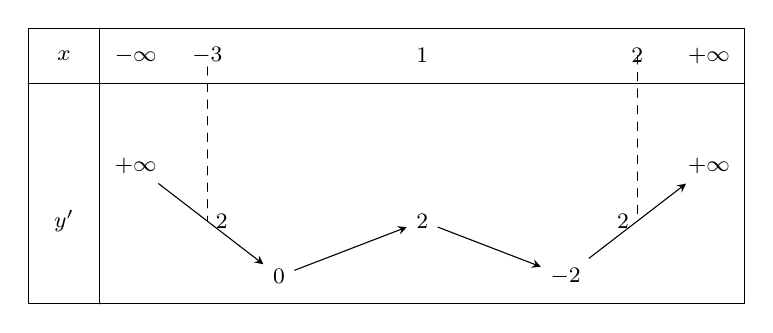
\begin{tikzpicture}[scale=0.7, font=\footnotesize, line join=round, line cap=round,>=stealth,yscale=1.0,xscale=1.3]
	\def\cot{9} % số nhãn chiều dài
	\def\hang{4} % số nhãn chiều cao
	\draw[shift={(-.5,.5)}] 
	(0,0) rectangle +(\cot+1,-\hang-1)
	(0,-1)--+(0:\cot+1) 
	(1,0)--+(-90:\hang+1);
	% \foreach \j in {0,...,\hang}
	% \foreach \i in {0,...,\cot}{
	%	\coordinate (\i\j) at (\i,-\j);
	%	\draw[gray!30]
	%	([xshift=-0.5cm,yshift=-0.5cm]\i\j)--([xshift=-0.5cm,yshift=-0.5cm]\i\j)--([xshift=-0.5cm,yshift=-0.5cm]\i\j)-- ([xshift=-0.5cm,yshift=-0.5cm]\i\j)--cycle
	%	(\i\j)node[]{\i\j};
	%}
	\path 
	(0,0) node{$x$}
	(1,0) node{$-\infty$}
	(2,0) node{$-3$}
	(5,0) node{$1$}
	(8,0) node{$2$}
	(9,0) node{$+\infty$}
	(0,-3) node{$y'$} 
	(1,-2) node (dvcL) {$+\infty$}
	(3,-4) node (CTL) {$0$} 
	(7,-4) node (CTR) {$-2$} 
	(5,-3) node (CD) {$2$} 
	(2.2,-3) node {2}
	(7.8,-3) node {2}
	(9,-2) node (dvcR) {$+\infty$} ;
	\draw[->] (dvcL)--(CTL);
	\draw[->] (CTL)--(CD);
	\draw[->] (CD)--(CTR);
	\draw[->] (CTR)--(dvcR);
	\draw[dashed,thin] (2,-0.2)--(2,-3) (8,0)--(8,-3);
	\end{tikzpicture}
	\end{center}
	Phương trình $f\left(\dfrac{1}{2} f(x)-1\right)=2 x+2$ có tối đa bao nhiêu nghiệm thực phân biệt?
	\choice
	{5}
	{4}
	{\True 3}
	{2}
	\loigiai{
	Đặt $t=\dfrac{1}{2} f(x)-1 \Leftrightarrow f(x)=2 t+2$ và phương trình trở thành $f(t)=2 x+2$
	$$
	\Rightarrow f(x)-f(t)=2 t-2 x \Leftrightarrow f(t)+2 t=f(x)+2 x(*)
	$$
	Hàm số $g(a)=f(a)+2 a$ có $g^{\prime}(a)=f^{\prime}(a)+2 \geq 0, \forall a \in \mathbb{R}$ (quan sát bảng biến thiên của $f^{\prime}(x)$ ) nên $g(a)$ đồng biến trên $\mathbb{R}$ do đó $(*) \Leftrightarrow g(t)=g(x) \Leftrightarrow t=x$\\
	Vậy đưa về phương trình $f(x)=2 x+2 \Leftrightarrow h(x)=f(x)-2 x-2=0$.\\
	Ta có $h^{\prime}(x)=f^{\prime}(x)-2=0 \Leftrightarrow f^{\prime}(x)=2 \Leftrightarrow x=-3 ; x=1 ; x=2$.\\
	Bảng biến thiên:
	\begin{center}
	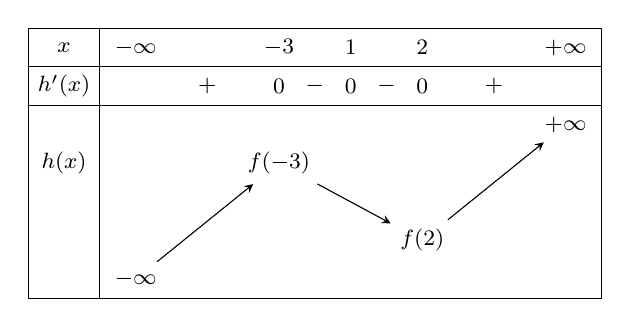
\begin{tikzpicture}[scale=0.7, font=\footnotesize, line join=round, line cap=round,>=stealth,yscale=.7,xscale=1.3]
	\def\cot{7} % số nhãn chiều dài
	\def\hang{6} % số nhãn chiều cao
	\draw[shift={(-.5,.5)}] 
	(0,0) rectangle +(\cot+1,-\hang-1)
	(0,-1)--+(0:\cot+1) 
	(0,-2)--+(0:\cot+1) 
	(1,0)--+(-90:\hang+1);
	% \foreach \j in {0,...,\hang}
	% \foreach \i in {0,...,\cot}{
	%	\coordinate (\i\j) at (\i,-\j);
	%	\draw[gray!30]
	%	([xshift=-0.5cm,yshift=-0.5cm]\i\j)--([xshift=-0.5cm,yshift=-0.5cm]\i\j)--([xshift=-0.5cm,yshift=-0.5cm]\i\j)-- ([xshift=-0.5cm,yshift=-0.5cm]\i\j)--cycle
	%	(\i\j)node[]{\i\j};
	%}
	\path 
	(0,0) node{$x$} 
	(1,0) node{$-\infty$}
	(3,0) node{$-3$}
	(5,0) node{$2$}
	(4,0) node {$1$}	 	
	(7,0) node{$+\infty$}	 	
	(0,-1) node{$h'(x)$}
	(2,-1) node{$+$}
	(3,-1) node{$0$}
	(3.5,-1) node {$-$}
	(4,-1) node{$0$}
	(4.5,-1) node {$-$}
	(5,-1) node{$0$}
	(6,-1) node{$+$}
	(0,-3) node{$h(x)$}
	(1,-6) node (avc) {$-\infty$}	
	(3,-3) node (CD) {$f(-3)$}
	(5,-5) node (CT) {$f(2)$}
	(7,-2) node (dvc) {$+\infty$};
	\draw[->] (avc)--(CD);
	\draw[->] (CD)--(CT);
	\draw[->] (CT)--(dvc);
	\end{tikzpicture}
	\end{center}
	Suy ra $h(x)=0$ có tối đa 3 nghiệm thực phân biệt. 
	}
\end{ex}
%%==========Câu 43
\begin{ex}%[2H3K3-3]
	Trong không gian $Oxyz$, cho hai đường thẳng $d_1\colon \dfrac{x-1}{1}=\dfrac{y+1}{-1}=\dfrac{z}{2}$; $d_2\colon \dfrac{x}{1}=\dfrac{y-1}{2}=\dfrac{z}{1}$. Đường thẳng $d$ đi qua $A\left(1;0;1\right)$ lần lượt cắt $d_2$, $d_2$ tại $B$ và $C$. Độ dài $BC$ bằng
	\choice
	{\True$\dfrac{7\sqrt{6}}{4}$}
	{$\dfrac{3\sqrt{3}}{2}$}
	{$\dfrac{5\sqrt{3}}{2}$}
	{$\dfrac{7\sqrt{6}}{2}$}
	\loigiai{
	Ta có $B\in d_1\Rightarrow B\left(1+b;-1-b;2b\right)$ và $C\in d_2\Rightarrow C\left(c;1+2c;c\right)$.\\
	Vì $d$ đi qua $A\left(1;0;1\right)$ lần lượt cắt $d_2$, $d_2$ tại $B$ và $C$ nên ta có $A, B, C$ thẳng hàng. Khi đó\\
	$\vec{AB}=k\vec{AC}\Leftrightarrow \left(b;-1-b;2b-1\right)=k\left(c-1;1+2c;c-1\right)\Leftrightarrow\heva{b&=&k(c-1)\\-1-b&=&k(1+2c)\\2b-1&=&k(c-1)}\Leftrightarrow\heva{b&=1\\kc&=-\dfrac{1}{3}\\k&=-\dfrac{4}{3}}\Leftrightarrow\heva{b&=1\\c&=\dfrac{1}{4}\\k&=-\dfrac{4}{3}.}$\\
	Do đó $B\left(2;-2;2\right)$, $C\left(\dfrac{1}{4};\dfrac{3}{2};\dfrac{1}{4}\right)\Rightarrow BC=\dfrac{7\sqrt{6}}{4}$.
	}
\end{ex}
%%==========Câu 44
\begin{ex}%[2D3K2-3]
	Cho hàm số $f(x)$ có đạo hàm $f^{\prime}(x)=xe^{x-a}$, $\forall x\in\mathbb{R}$ và $f(0)=-e^{-a}-1$ (với $a$ là tham số thực). Khi $\displaystyle\int\limits_0^a f(x) \mathrm{\,d}x=4$, khẳng định nào dưới đây đúng?
	\choice
	{\True $a\in\left(-2;-1\right)$}
	{$a\in\left(-1;0\right)$}
	{$a\in\left(0;1\right)$}
	{$a\in\left(1;2\right)$}
	\loigiai{
	Ta có $\displaystyle\int f^{\prime}(x) \mathrm{\,d}x=\displaystyle\int xe^{x-a} \mathrm{\,d}x$.
	Đặt $\heva{&u=x\\& \mathrm{\,d}v=e^{x-a}}\Rightarrow\heva{&\mathrm{\,d}u=\mathrm{\,d}x\\&v=e^{x-a}}$.\\
	$\Rightarrow f(x)=\displaystyle\int xe^{x-a} \mathrm{\,d}x=xe^{x-a}-\displaystyle\int e^{x-a} \mathrm{\,d}x=xe^{x-a}-e^{x-a}+C$.\\
	Vì $f(0)=-e^{-a}-1\Rightarrow C=-1$ nên $f(x)=xe^{x-a}-e^{x-a}-1$.\\
	Do đó $\displaystyle\int\limits_0^a f(x) \mathrm{\,d}x=\displaystyle\int\limits_0^a \left(xe^{x-a}-e^{x-a}-1\right) \mathrm{\,d}x=\displaystyle\int\limits_0^a xe^{x-a} \mathrm{\,d}x-\displaystyle\int\limits_0^a e^{x-a} \mathrm{\,d}x-\displaystyle\int\limits_0^a \mathrm{\,d}x=$\\
	$=\left(xe^{x-a}-2e^{x-a}-x \right)\bigg|_0^a= -2+2e^{-a}=4\Leftrightarrow e^{-a}=3\Leftrightarrow a=-\ln3\approx -1{,}09\in \left(-2;-1\right)$.
	}
\end{ex}
%%==========Câu 45
\begin{ex}%[2H3G2-7]
	Trong không gian $Oxyz$, cho mặt cầu $(S)\colon (x-2)^2+(y-3)^2+(z-1)^2=\dfrac{1}{2}$. Có bao nhiêu cặp số nguyên $(a ; b)$ sao cho tồn tại hai điểm $A(a ; 0 ; 0)$ và $B(0 ; b ; 0)$ để có hai mặt phẳng vuông góc với nhau cùng đi qua $A$, $B$ và tiếp xúc với $(S)$?
	\choice
	{$5$}
	{$7$}
	{\True $8$}
	{$6$}
	\loigiai{
	\immini{
	Mặt cầu đã cho có tâm $I=(2 ; 3 ; 1)$, $R=\dfrac{1}{\sqrt{2}}$.\\
	Gọi hai mặt phẳng qua $A$, $B$ và tiếp xúc với $(S)$ tại $M$, $N$.\\
	Goi $H$ là hình chiếu của $I$ lên $AB \Rightarrow \heva{&A B \perp I H, A B \perp I M \Rightarrow A B \perp(I H M) \\& A B \perp I H, A B \perp I N \Rightarrow A B \perp(I H N).}$\\
	$ \Rightarrow(I H M) \equiv(I H N)$ và $((M A B),(N A B))=(H M, H N)$.\\
	Vì $((M A B),(N A B))=90^{\circ} \Rightarrow \widehat{M H N}=90^{\circ}\\ \Rightarrow M I N H$ là hình vuông do đó $I H=\sqrt{2} R=1$.\\
	Ta có $\overrightarrow{A B}=(-a ; b ; 0)$, $\overrightarrow{I A}=(a-2 ;-3 ;-1) \Rightarrow\left[\overrightarrow{A B}, \overrightarrow{I A}\right]=(-b ;-a ; 3 a+2 b-a b)$.\\
	$\Rightarrow I H=\mathrm{d}(I, A B)=\dfrac{\left|[\overrightarrow{A B}, \overrightarrow{I A}]
	\right|
	}{\left|\overrightarrow{A B}\right|}=1 \Leftrightarrow \dfrac{b^2+a^2+(3 a+2 b-a b)^2}{a^2+b^2}=1$\\
	$\Leftrightarrow 3 a+2 b-a b=0 \Leftrightarrow b(a-2)=3 a \Rightarrow b=\dfrac{3 a}{a-2}=\dfrac{3(a-2)+6}{a-2}=3+\dfrac{6}{a-2} \in \mathbb{Z}$.\\
	$\Rightarrow a-2 \in\{ \pm 1, \pm 2, \pm 3, \pm 6\} \Rightarrow 8$ cặp số nguyên $(a ; b)$ thoả mãn.
	}
	{\begin{tikzpicture}[scale=0.7, font=\footnotesize, line join=round, line cap=round, >=stealth]
	\coordinate (I) at (0,4);
	\coordinate (N) at (2,4);
	\coordinate (M) at (0,0);
	\coordinate (A) at (3.5,-2.5);
	\coordinate (B) at (5,0);
	\coordinate (H) at ($(A)!0.4!(B)$);
	\draw (A) node[below]{$A$}--(B) node[right]{$B$} (A)--(M) node[left]{$M$}--(I) node[above right]{$I$}--(N) node[above right]{$N$}--(H) (B)--(N)--(A)--(I);
	\draw[dashed] (M)--(H)node[below right]{$H$} (M)--(B)--(I)--(H);
	\end{tikzpicture}}
	\noindent
	Nhận xét: Nếu đề bài yêu cầu hai điểm $A$ và $B$ phân biệt hoặc có đúng hai mặt phẳng vuông góc với nhau cùng đi qua $A, B$ và tiểp xúc với ( $S$ ) thỉ các em loại đi trường hợp $A, B$ trùng nhau tức cặp $(a ; b)=(0 ; 0)$.
	}
\end{ex}
%%==========Câu 46
\begin{ex}%[2H1K3-2]
	Cho khối chóp $S.ABCD$ có đáy $ABCD$ là hình bình hành tâm $O$, $AB=a$, $BC=2a$ và $\widehat{A B C}=60^{\circ}$. Hình chiếu vuông góc của đỉnh $S$ trên mặt phẳng $(ABCD)$ là điểm $O$. Biết hai mặt phẳng $(SAB)$ và $(SCD)$ vuông góc với nhau, thể tích của khối chóp đã cho bằng
	\choice
	{$\dfrac{\sqrt{21} a^3}{6}$}
	{$\dfrac{\sqrt{3} a^3}{6}$}
	{$\dfrac{\sqrt{3} a^3}{3}$}
	{\True $\dfrac{a^3}{2}$}
	\loigiai{
	\begin{center}
	\begin{tikzpicture}[scale=0.7,>=stealth, font=\footnotesize, line join=round, line cap=round]	%hình chóp có đáy là hình thang.
	\coordinate[label=above right:$A$] (A) at (0,0);
	\coordinate[label=below left:$B$] (B) at (-4,-3);
	\coordinate[label=below left:$C$] (C) at (4,-3);
	\coordinate[label=right:$D$] (D) at (8,0);
	\coordinate[label=above:$S$] (S) at ($(A)+(2,4)$);
	\coordinate[label=below:$O$] (O) at ($(B)!1/2!(D)$);
	\coordinate[label=right:$N$] (N) at ($(C)!1/3!(D)$);
	\coordinate[label=left:$M$] (M) at ($(A)!1/3!(B)$);
	\coordinate[label=below right:$H$] (H) at ($(A)!2/3!(B)$);
	\draw (S)--(B)--(C)--(D)--(S)--(C) (S)--(N);
	\draw[dashed] (C)--(A)--(B) (S)--(A)--(D) (B)--(D) (S)--(O) (C)--(H) (M)--(N) (S)--(M);
	\foreach \diem in {A,B,C,D,S,O,M,H,N}	\fill (\diem)circle(1.5pt);
	\end{tikzpicture}
	\end{center}
	\begin{itemize}
	\item Cách 1\\	
	Ta có $O=A C \cap B D \Rightarrow SO \perp(A B C D)$ và $S_{A B C D}=2 S_{A B C}=BA \cdot BC \cdot \sin \widehat{A B C}=\sqrt{3} a^2$.\\
	Và $AB\parallel CD$ ; $AB \subset(S A B)$; $CD \subset (S C D) \Rightarrow (S A B) \cap(S C D)=Sx\parallel A B \parallel C D$.\\
	Kẻ đường thẳng qua $O$ vuông góc với $A B$, $CD$ lần lượt tại $M$, $N \Rightarrow S x\parallel A B\parallel CD \perp(S M N)$.\\
	Khi đó $((S A B),(S C D))=(S M, S N)=90^\circ \Leftrightarrow \widehat{M S N}=90^{\circ} \Rightarrow S O=\dfrac{M N}{2}=\dfrac{C H}{2}=\dfrac{C B\cdot \sin 60^\circ}{2}=\dfrac{\sqrt{3} a}{2}$.\\
	Khi đó $V_{S.A B C D}=\dfrac{1}{3} S_{A B C D} \cdot S O=\dfrac{1}{3} \cdot \sqrt{3} a^2 \cdot \dfrac{\sqrt{3}\cdot a}{2}=\dfrac{a^3}{2}$.
	\item 
	Cách 2\\ Nếu các em gắn trục tọa độ $Oxyz$ thì chỉ ra $A B=a$, $B C=2 a$, $\widehat{A B C}=60^{\circ} \Rightarrow A C=\sqrt{3} a \Rightarrow A B \perp A C$.\\
	Chọn hệ trục toạ độ $O x y z$ sao cho $O x$, $O y$ lần lượt trủng với các tia $A B$, $A C$ và $O z$ qua $A$ củng hướng với tia $O S$.\\
	Khi đó toạ độ các điểm là $A(0 ; 0 ; 0)$, $B(1 ; 0 ; 0)$, $C(0 ; \sqrt{3} ; 0)$;\\ $\overrightarrow{A D}=\overrightarrow{B C}=(-1 ; \sqrt{3} ; 0) \Rightarrow D(-1 ; \sqrt{3} ; 0)$ và $O\left(0 ; \dfrac{\sqrt{3}}{2} ; 0\right) \Rightarrow S\left(0 ; \dfrac{\sqrt{3}}{2} ; h\right)$.\\
	Ta có $\overrightarrow{n}_{(S A B)}=[\overrightarrow{A B}, \overrightarrow{A S}]=\left(0 ;-h ; \dfrac{\sqrt{3}}{2}\right), \overrightarrow{n}_{(S C D)}=[\overrightarrow{S C}, \overrightarrow{S D}]=\left(0 ; h ; \dfrac{\sqrt{3}}{2}\right)$.\\
	Vậy $(S A B) \perp(S C D) \Leftrightarrow-h^2+\dfrac{3}{4}=0 \Rightarrow h=\dfrac{\sqrt{3}}{2} \Rightarrow S O=\dfrac{\sqrt{3}}{2}\\ \Rightarrow V_{S.A B C D}=\dfrac{1}{3} S_{A B C D} \cdot S O=\dfrac{1}{3} \cdot \sqrt{3} a^2 \cdot \dfrac{\sqrt{3} a}{2}=\dfrac{a^3}{2}$.
	\end{itemize}
	}
\end{ex}
%%==========Câu 47
\begin{ex}%[2D3G3-1]
	Cho đường thẳng $d\colon y=g(x)$ cắt đồ thị hàm số bậc ba $f(x)$ tại ba điểm phân biệt có hoành độ là $x_1$, $x_2$, $x_3$, $\left(x_1<x_2<x_3\right)$. Gọi $S_1$ là diện tích hình phẳng giới hạn bởi các đường $y=f(x)$; $y=g(x)$; $x=x_1$; $x=x_2$ và $S_2$ là diện tích hình phẳng giới hạn bởi các đường $y=f(x)$ ; $y=g(x)$; $x=x_2$; $x=x_3$. Khi $S_1=2 S_2$ thì $\dfrac{x_1-x_2}{x_2-x_3}$ thuộc khoảng nào dưới đây?
	\choice
	{\True $ \left(1;\dfrac{4}{3}\right) $}
	{$ \left(\dfrac{4}{3};\dfrac{3}{2}\right) $}
	{$ \left(\dfrac{3}{2};\dfrac{8}{5}\right) $}
	{$ \left(\dfrac{8}{5};2\right) $}
	\loigiai{
	Theo giả thiết có $f(x)-g(x)=k(x-a)(x-b)(x-c)$, $(a<b<c)$ ở đây $x_1=a$; $x_2=b$; $x_3=c$ để thao tác cho gọn. Giả sử $k>0$ ta cần tính $t=\dfrac{a-b}{b-c}$, $(t>0)$.\\ 
	Ta có $S_1=k \displaystyle\int\limits_a^b(x-a)(x-b)(x-c) \mathrm{\,d}x=\dfrac{k}{12}(a-b)^3(a+b-2 c)$ và\\ $S_2=-k \displaystyle\int\limits_b^c (x-a)(x-b)(x-c) \mathrm{\,d} x=-\dfrac{k}{12}(b-c)^3(b+c-2 a)$.\\
	Suy ra $$\dfrac{S_1}{S_2}=\dfrac{a+b-2 c}{2 a-b-c}\left(\dfrac{a-b}{b-c}\right)^3=\dfrac{(a-b)+2(b-c)}{2(a-b)+(b-c)}\left(\dfrac{a-b}{b-c}\right)^3=2 \Leftrightarrow \dfrac{t+2}{2 t+1} t^3=2 \Leftrightarrow t^4+2 t^3-4 t-2=0 \Rightarrow t \approx 1{,}2966.$$
	Để tính $S_1$, $S_2$ các em thực hiện như sau:\\
	Đã biết $\quad \displaystyle\int\limits_a^b(x-a)(x-b) \mathrm{\,d} x=\dfrac{1}{6}(a-b)^3$ ;\\ $\mathrm{\,d}[(x-a)(x-b)]=(2 x-(a+b)) \mathrm{\,d} x \quad$ vậy phân tích $ x-c=\dfrac{1}{2}[(2 x-(a+b))+(a+b-2 c)]$ khi đó
	\begin{eqnarray*}
	&\dfrac{S_1}{k}&=\dfrac{1}{2} \displaystyle\int\limits_a^b(x-a)(x-b)(2 x-(a+b)) \mathrm{\,d} x+\dfrac{1}{2}(a+b-2 c) \displaystyle\int\limits_a^b(x-a)(x-b) \mathrm{\,d} x\\
	& &= \dfrac{1}{2} \displaystyle\int\limits_a^b(x-a)(x-b) \mathrm{\,d}[(x-a)(x-b)]+\dfrac{1}{2}(a+b-2 c) \cdot \dfrac{1}{6}(a-b)^3\\
	& &= \left.\dfrac{1}{4}[(x-a)(x-b)]^2 \right|^a_b+\dfrac{1}{12}(a-b)^3(a+b-2 c)=\dfrac{1}{12}(a-b)^3(a+b-2 c).
	\end{eqnarray*}
	để tính $S_2$ chỉ việc thay đổi vai trò $a$, $b$ trong $S_1$ lần lượt bởi $b$, $c$ ta có $S_2=-\dfrac{k}{12}(b-c)^3(b+c-2 a)$.
	}
\end{ex}
%%==========Câu 48
\begin{ex}%[2D1G5-5]
	Cho hàm số $f(x)$ có đạo hàm xác định và liên tục trên $\mathbb{R}$, hình vẽ bên là đồ thị của hai hàm số $y=f(x)$ và $y=f'(x)$.
	\begin{center}
	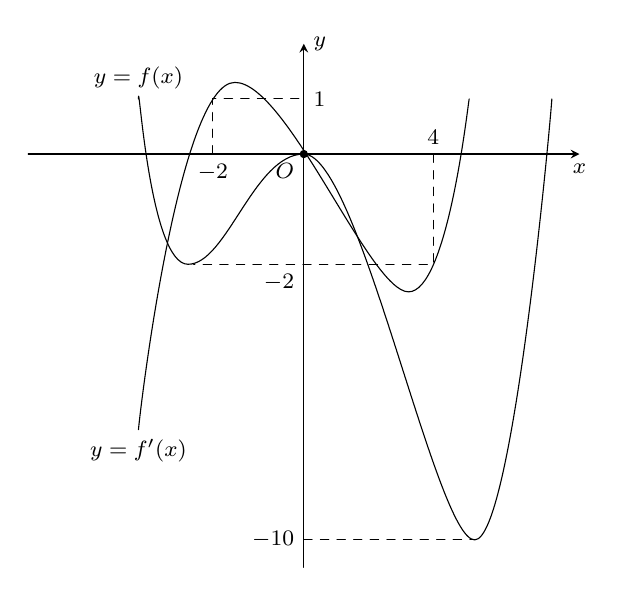
\begin{tikzpicture}[>=stealth, line join=round, line cap=round, font=\footnotesize, scale=1,x=.7cm,y=.7cm]
	\draw[->] (0,-7.5)--(0,2)node[right]{$y$};
	\draw[->] (-5,0)--(5,0)node[below]{$x$};
	\fill (0,0)node[below left]{ $O$}circle(1.5pt);
	\path (-3,1) node[above]{$y=f(x)$};
	\path (-3,-5) node[below]{$y=f'(x)$};
	\draw[dashed] (2.35,0)node[above]{$4$} |-(0,-2)node[below left]{$-2$}--++(180:2)
	(-1.65,0)node[below]{$-2$}|-(0,1)node[right]{$1$}
	(0,-7)node[left]{$-10$}--++(0:3.1);
	\draw
	(-3,1).. controls +(90:.5) and +(180:.7)..
	(-2.1,-2) .. controls +(0:.7) and +(180:.9)..
	(0,0) .. controls +(0:1) and +(180:.7)..
	(3.1,-7) .. controls +(0:.7) and +(-92:.2)..
	(4.5,1)
	;
	\draw
	(-3,-5) ..controls +(85:.5) and +(180:1)..
	(-1.25,1.3) ..controls +(0:.95) and +(180:.7)..
	(1.9,-2.5) ..controls +(0:.7) and +(-100:.2)..
	(3,1)
	;
	\end{tikzpicture}
	\end{center}
	Tổng các giá trị nguyên của tham số $m$ để hàm số $g(x)=f[f(x)-m+1]+\dfrac{1}{4}[f(x)-m+1]^2$ có $ 11 $ điểm cực trị là
	\choice
	{$ 3 $}
	{\True $ -2 $}
	{$ 4 $}
	{$ -1 $}
	\loigiai{
	Ta có yêu cầu bài toán $\Leftrightarrow g'(x)=f'(x)\left[f'(f(x)-m+1)+\dfrac{1}{2}(f(x)-m+1)\right]$ có 11 lần đổi dấu\\
	$\Leftrightarrow f'\left[f(x)-m+1\right]+\dfrac{1}{2}(f(x)-m+1)$ có 8 lần đổi dấu.\\
	Vẽ thêm đường thẳng $y=-\dfrac{x}{2}$ qua các điểm $(-2 ; 1)$; $(0 ; 0)$; $(4 ;-2)$ suy ra $f'(x)+\dfrac{1}{2} x$ cùng dấu với $(x+2) x(x-4)$.
	\begin{center}
	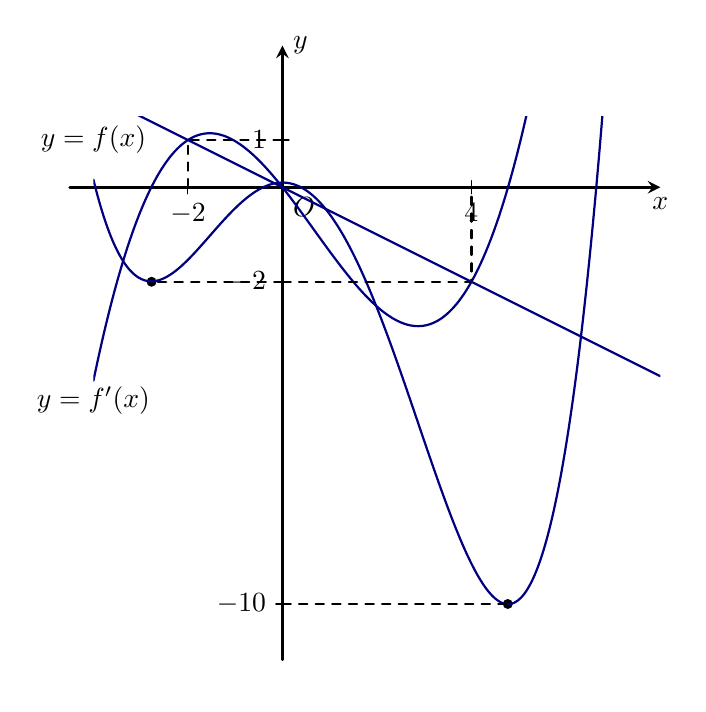
\begin{tikzpicture}[line join = round, line cap = round,>=stealth,thick,scale=.6] 
	%Vẽ hệ trục Oxy 
	\draw[->,line width = 1pt] (-4.5,0)--(0,0) node[below right]{$O$}--(8,0) node[below]{$x$}; 
	\draw[->,line width = 1pt] (0,-10)--(0,3) node[right]{$y$}; 
	%Vẽ các điểm trên hệ trục 
	\foreach \x in {-2,4} \draw[thin] (\x,4pt)--(\x,-4pt) node [below] {$\x$}; 
	\foreach \y in {-2,1} \draw[thin] (4pt,\y)--(-4pt,\y) node [left] {$\y$};
	\path (-4,0.5) node[above]{$y=f(x)$};
	\path (-4,-4) node[below]{$y=f'(x)$};
	\fill[black] (-2.77,-2) circle (3pt);
	\fill[black] (4.77,-8.82) circle (3pt);
	\draw[thin] (4pt,-8.82)--(-4pt,-8.82) node [left] {$-10$};
	\clip (-4,-10.5) rectangle (8,1.5);
	%Vẽ đồ thị hàm số 
	\draw[samples=200,domain=-4:6,smooth,blue!50!black] plot (\x, {(2/21)*(\x)^3-(4/21)*(\x)^2-(53/42)*\x}); 
	\draw[samples=200,domain=-4:8,smooth,blue!50!black] plot (\x, {(1/42)*(\x)^4-(4/63)*(\x)^3-(53/84)*(\x)^2+0.1}); 
	\draw[dashed] (0,-2)--(4,-2)--(4,0) (-2,0)--(-2,1)--(0,1) (0,-2)--(-2.77,-2) (0,-8.82)--(4.77,-8.82);
	\draw[samples=200,domain=-4:8,smooth,blue!50!black] plot (\x, {-(1/2)*(\x)}); 
	\end{tikzpicture}
	\end{center}
	Do đó $f'(f(x)-m+1)+\dfrac{1}{2}(f(x)-m+1)$ cùng dấu với $(f(x)-m+3)(f(x)-m+1)(f(x)-m-3)$.\\
	Xét $(f(x)-m+3)(f(x)-m+1)(f(x)-m-3)=0 \Leftrightarrow\hoac{&f(x)-3=m \\ &f(x)+1=m \\ &f(x)+3=m.}$\\
	Vẽ bảng biến thiên của ba hàm số $y=f(x)-3$; $y=f(x)+1$; $y=f(x)+3$.
	\begin{center}
	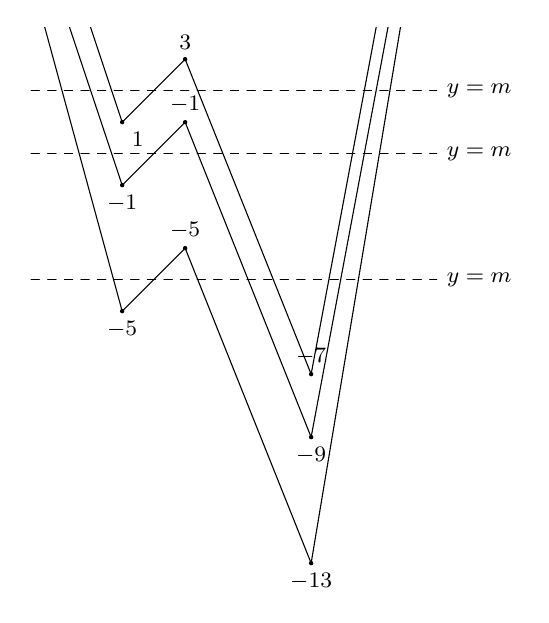
\begin{tikzpicture}[line join = round, line cap = round,>=stealth,font=\footnotesize,scale=.4]
	\path (10,0) node[right]{$y=m$};
	\path (10,2) node[right]{$y=m$};
	\path (10,-4) node[right]{$y=m$};
	\clip (-3,-14) rectangle (10,4);
	\coordinate(D1) at (-3,10);
	\coordinate(D2) at (-3,8);
	\coordinate(D3) at (-3,6);
	\coordinate[label=below right :$1$](A1) at (0,1);
	\coordinate[label=below :$-1$](A2) at (0,-1);
	\coordinate[label=below:$-5$](A3) at (0,-5);
	\coordinate[label=above :$3$](B1) at (2,3);
	\coordinate[label=above :$-1$](B2) at (2,1);
	\coordinate[label=above:$-5$](B3) at (2,-3);
	\coordinate[label=above:$-7$](C1) at (6,-7);
	\coordinate[label=below :$-9$](C2) at (6,-9);
	\coordinate[label=below:$-13$](C3) at (6,-13);
	\coordinate(E1) at (9,9);
	\coordinate(E2) at (9,7);
	\coordinate(E3) at (9,5);
	\fill[black] (A1) circle (2pt) (B1) circle (2pt) (C1) circle (2pt) (A2) circle (2pt) (B2) circle (2pt) (C2) circle (2pt) (A3) circle (2pt) (B3) circle (2pt) (C3) circle (2pt);
	\draw (D1)--(A1)--(B1)--(C1)--(E1) (D2)--(A2)--(B2)--(C2)--(E2) (D3)--(A3)--(B3)--(C3)--(E3);
	\draw [dashed](-5,2)--(10,2) (-5,0)--(10,0) (-5,-4)--(10,-4);
	\end{tikzpicture}
	\end{center}
	Suy ra điều kiện là $\hoac{&-5<m<-3 \\ &-1<m<1 \\& 1<m<3} \Rightarrow m \in\{-4,0,2\} \Rightarrow \displaystyle\sum m=-4+0+2=-2$.\\
	\textbf{Cách 2:} Xét $h(x)=f(x)+\dfrac{1}{4} x^2 ; u(x)=f(x)-m+1 \Rightarrow g(x)=h[u(x)]$.\\
	Ta có $h'(x)=f'(x)+\dfrac{x}{2}=0 \Leftrightarrow f'(x)=-\dfrac{x}{2} \Leftrightarrow \hoac{&x=-2 \\ &x=0 \\ &x=4} \Rightarrow h(x)$ có ba điểm cực trị $\hoac{&x=-2 \\ &x=0 \\ &x=4.}$\\
	Hàm số $u(x)=f(x)-m+1$ có ba điểm cực trị nên ycbt $\Leftrightarrow h'[u(x)]$ đổi dấu $11-3=8$ lần $\Leftrightarrow(u(x)+2) u(x)(u(x)-4)$ đổi dấu 8 lần, các bước sau thực hiện tương tự cách 1.
	}
\end{ex}
%%==========Câu 49
\begin{ex}%[2D2G5-5]
	Có bao nhiêu số nguyên $x$, $(x\ge-20)$ sao cho ứng với mỗi $x$ tồn tại đúng hai cặp số thực $(y;z)$ thỏa mãn $\log_2\left(2y^2+z^2\right)=\log_3\left(y^3+2z^3\right)=x$?
	\choice
	{$29$}
	{$21$}
	{\True $32$}
	{$22$}
	\loigiai{
	Ta có $\left\{\begin{aligned}
	&2 y^2+z^2=2^x \\
	& y^3+2 z^3=3^x\end{aligned} \Rightarrow \dfrac{\left(2 y^2+z^2\right)^3}{\left(y^3+2 z^3\right)^2}=\left(\dfrac{8}{9}\right)^x\right.$.\\
	Mặt khác $\dfrac{\left(2 y^2+z^2\right)^3}{\left(y^3+2 z^3\right)^2}=g(a)=\dfrac{\left(2 a^2+1\right)^3}{\left(a^3+2\right)^2},\left(a=\dfrac{y}{z}\right)$.\\
	Ta có $g^{\prime}(a)=\dfrac{12 a\left(2 a^2+1\right)^2\left(a^3+2\right)^2-6 a^2\left(a^3+2\right)\left(2 a^2+1\right)^3}{\left(a^3+2\right)^4}=\dfrac{6 a\left(2 a^2+1\right)^2(4-a)}{\left(a^3+2\right)^3}$.\\
	Bảng biến thiên
	\begin{center}
	
\begin{tikzpicture}[>=stealth]
	\tkzTabInit[nocadre=false,lgt=1.2,espcl=2,deltacl=.6] {$a$/.6, $g’(a)$/.6,$g(a)$/2}
	{$-\infty$ , $-\sqrt[3]{2}$ , $0$ , $4$ , $+\infty$}
	\tkzTabLine{,+,d,-, $0$ ,+,$0$,-,}
	\tkzTabVar{-/$8$ ,+D+/$+\infty$/$+\infty$, -/$\dfrac{1}{3}$,+/$\dfrac{33}{4}$,-/$8$}
	\end{tikzpicture}
	\end{center}	
	Suy ra $\hoac{&\dfrac{1}{4}<\left(\dfrac{8}{9}\right)^x \leq 8 \\& \left(\dfrac{8}{9}\right)^x>\dfrac{33}{4}} \Rightarrow x \in\{-20; \ldots; 11\}$.
	}
\end{ex}
%%==========Câu 50
\begin{ex}%[2D4G5-1]
	Xét hai số phức $z_1$, $z_2$ thảo mãn $\left|z_1\right|=\left|z_2-4-4i\right|=\dfrac{1}{2}$ và số phức $z$ thỏa mãn $|2z+2-5i|=|2z+3-6i|4$. Giá trị nhỏ nhất của biểu thức $P=\left|z-3z_1-\overline{z_1}\right|+\left|z-z_2\right|$ bằng
	\choice
	{$\dfrac{17}{2}$}
	{\True $\dfrac{13}{2}$}
	{$\dfrac{11}{2}$}
	{$\dfrac{15}{2}$}
	\loigiai{
	Đặt $z=x+yi$, $(x, y \in \mathbb{R})$\\
	\allowdisplaybreaks
	\begin{eqnarray*}
	\Rightarrow|2 z+2-5 i|=|2 z+3-6 i|
	&\Leftrightarrow &(2 x+2)^2+(2 y-5)^2=(2 x+3)^2+(2 y-6)^2\\
	&\Leftrightarrow& x-y+4=0\\
	& \Rightarrow& M(z) \in d\colon x-y+4=0.
	\end{eqnarray*}
	và $\left|z_2-4-4 i\right|=\dfrac{1}{2} \Rightarrow A\left(z_2\right) \in(C)$ có tâm $I(4 ; 4)$, $R=\dfrac{1}{2}$.\\
	Đặt $z_1=a+b i$, $(a, b \in \mathbb{R}) \Rightarrow\left|z-3 z_1-\overline{z_1}\right|=|z-(4 a+2 b i)|=M B$, $B(4 a+2 b i)$.\\
	Vì $\left|z_1\right|=\dfrac{1}{2} \Leftrightarrow a^2+b^2=\dfrac{1}{4} \Leftrightarrow \dfrac{x_B^2}{16}+\dfrac{y_B^2}{4}=\dfrac{1}{4} \Leftrightarrow \dfrac{x_B^2}{4}+\dfrac{y_B^2}{1}=1 \\
	\Rightarrow B \in(E)$ có độ dài trục lớn $2 a=4 ;$ độ dài trục nhỏ $2 b=2$.
	\begin{center}
	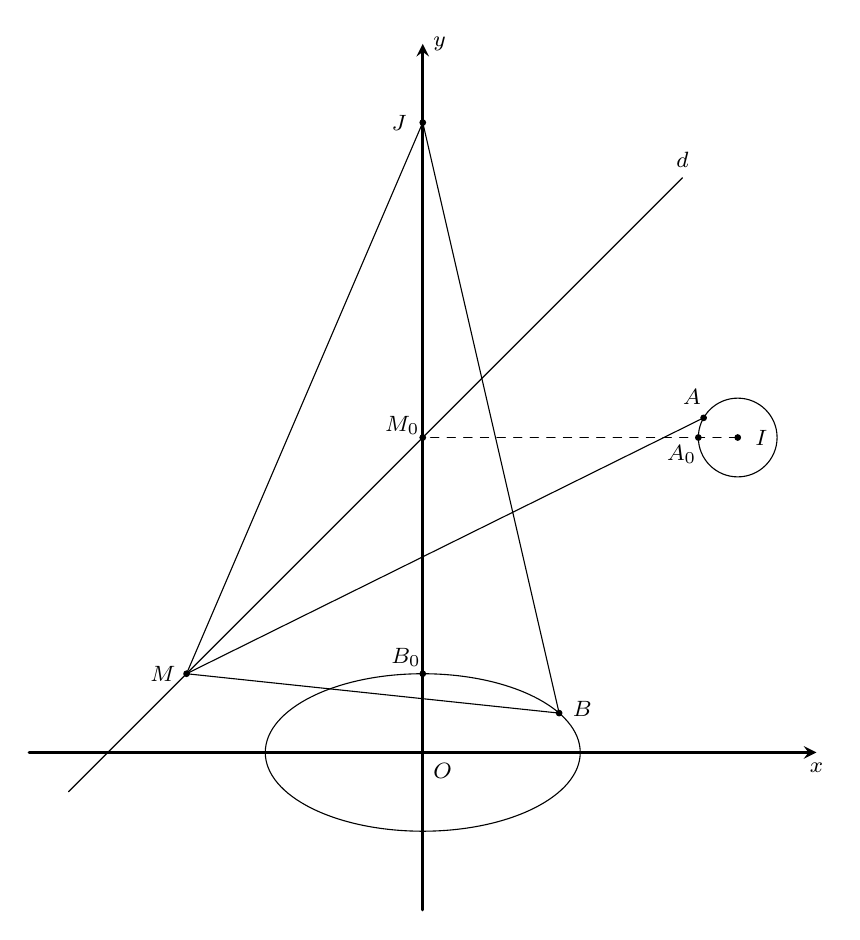
\begin{tikzpicture}[scale=1,>=stealth, font=\footnotesize, line join=round, line cap=round]
	\draw[->,line width=1pt] (-5,0)--(0,0) node[below right]{$O$}--(5,0) node[below]{$x$};
	\draw[->,line width=1pt] (0,-2)--(0,9) node[right]{$y$};
	%Vẽ elip trục lớn bằng 4, trục nhỏ bằng 2
	\draw (180:2) arc (180:0:{2} and {1});
	\draw (180:2)arc(180:360:{2} and {1})--cycle;
	\draw[smooth,samples=100] plot[domain=-4.5:3.3](\x,{(\x)+4})node[above]{$d$};
	\path 
	(0,8) coordinate (J) 
	(0,1) coordinate (B_0) 
	(4,4) coordinate (I)
	(180:2) arc (180:30:{2} and {1}) coordinate (B)
	(-3,1) coordinate (M)
	(0,4) coordinate (M_0)
	(3.5,4) coordinate (A_0)
	(3.5,4) arc (180:150:0.5) coordinate (A)
	;
	\draw (I) circle (0.5)
	(M)--(B)--(J)--cycle (A)--(M)
	;
	\draw[dashed] (I)--(M_0);
	\foreach \p/\g in {I/0, J/180, B_0/135, B/10, M/180, M_0/150, A_0/-135, A/120}
	\draw[fill=black] (\p) circle (1pt) node[shift=(\g:3mm)] {$\p$};
	\end{tikzpicture}
	\end{center}
	Khi đó $\begin{aligned}[t]P=M A+M B \geq(M I-I A)+M B&=(M I-R)+M B=(M I+M B)-\dfrac{1}{2}\\
	&=(M J+M B)-\dfrac{1}{2} \geq J B-\dfrac{1}{2} \geq J B_0-\dfrac{1}{2}\\
	&=8-1-\dfrac{1}{2}=\dfrac{13}{2}\end{aligned}$ \\
	trong đó $J(0 ; 8)$; $B_0(0 ; 1)$.\\
	Dấu bằng xảy ra khi $B \equiv B_0$; $M \equiv M_0$; $A \equiv A_0$.
	}
\end{ex}
\Closesolutionfile{ans}
\inputansbox{10}{ans/ans-Vted-20-2023}